\documentclass[11pt,a4j]{jarticle}

\newcommand{\setcounters}[1] {
  \setcounter{equation}{#1}
  \setcounter{figure}{#1}
  \setcounter{table}{#1}
}

\newcommand{\unit}[1] {
  \hspace{1mm}\mathrm{[#1]}
}

\newcommand{\degc} {
  \hspace{1mm}\mathrm{[}{}^\circ\mathrm{C]}
}

\newcommand{\refig}[1]{図\ref{fig::#1}}
\newcommand{\refeq}[1]{式(\ref{eq::#1})}
\newcommand{\reftab}[1]{表\ref{tab::#1}}

\newcommand{\fig}[5] {
  \begin{figure}[#1]
    \begin{center}
      \includegraphics[width=#2\hsize]{#3}
    \end{center}
    \caption{#4}
    \label{fig::#5}
  \end{figure}
}

\makeatletter
\def\eq{\@ifstar\@eq\@@eq}
\def\@eq#1{\begin{equation*}#1\end{equation*}}
\def\@@eq#1#2{\begin{equation}#2\label{eq::#1}\end{equation}}
\makeatother

\newcommand{\diff}[2] {
  \frac{\mathrm{d}#1}{\mathrm{d}#2}
}

\newcommand{\pdiff}[2] {
  \frac{\partial #1}{\partial #2}
}


\newcommand{\ddt}[2][1] {
  \ifnum #1 < 2
    \frac{\mathrm{d}#2}{\mathrm{d}t}
  \else
    \frac{\mathrm{d}^#1#2}{\mathrm{d}t^#1}
  \fi
}

\newcommand{\e}[1] {
  \mathrm{e}^{#1}
}

\newcommand{\lparen}{(}
\catcode `( = \active
\newcommand{(}{\ifmmode\left\lparen\else\lparen\fi}

\newcommand{\rparen}{)}
\catcode `) = \active
\newcommand{)}{\ifmmode\right\rparen\else\rparen\fi}

\newcommand{\bmat}[1] {
  \begin{bmatrix} #1 \end{bmatrix}
}

% -- Package ---------------------------------------------------
\usepackage[dvipdfmx]{graphicx}
\usepackage{amsmath, amssymb}
\usepackage{bm}
\usepackage{fancyhdr}
\usepackage{here}
\usepackage{listings}
\usepackage{multirow}


% -- Margin Config ---------------------------------------------
\setlength{\textheight}{\paperheight}
\setlength{\topmargin}{4.6truemm} % 30mm(=1.0in+4.6mm)
\addtolength{\topmargin}{-\headheight}
\addtolength{\topmargin}{-\headsep}
\addtolength{\textheight}{-60truemm}

\setlength{\textwidth}{\paperwidth}
\setlength{\oddsidemargin}{-0.4truemm} % 25mm(=1.0in-0.4mm)
\setlength{\evensidemargin}{-0.4truemm}
\addtolength{\textwidth}{-50truemm}


% -- Renewcommand ----------------------------------------------
\renewcommand{\theequation}{\arabic{section}.\arabic{equation}}
\renewcommand{\thefigure}{\thesection.\arabic{figure}}
\renewcommand{\thetable}{\thesection.\arabic{table}}
\renewcommand{\lstlistingname}{ソースコード}
\renewcommand{\headrulewidth}{0mm} % fancy
\renewcommand{\labelenumi}{(\arabic{enumi})}


% -- Config for fancy package ----------------------------------
\pagestyle{fancy}
\rhead{\thepage}
\lhead{}
\cfoot{}


% -- Config for package listings -------------------------------
\lstset{
  basicstyle={\ttfamily \small},
  breaklines=true,
  frame=trBL,
  numbers=left,
  numberstyle={\ttfamily \small},
}




\begin{document}
\section{機体の再設計}
\subsection{前回の反省}
前回のレポートで紹介した機体を図\ref{kuwano1}に示す.これを一号機とし,
一号機での反省点を元に再設計した機体を二号機とした.
二号機の概要を図\ref{kuwano2}に示す.一号機での反省点を以下に述べる.

\begin{itemize}
 \item 車体に無駄なスペースが多い.
 \item 車体の幅が大きい.
 \item 回路のガードがされていない.
\end{itemize}

西田研では,これらの反省点を改善するために,機体の大幅な見直しを行った.
改善した点について以下に述べていく.

\subsection{モータとエンコーダの配置}
一号機の駆動系を図\ref{kuwano3}に示す.一号機では,
モータとエンコーダの配置を線対称としていたため,
機体の幅が大きくしなければならなかった.そこで,
二号機ではこのモータとエンコーダの配置を点対象とすることにした.
これにより,タイヤのトレッド幅を限りなく小さくでき,
機体の幅を小さくすることができた.
また,一号機ではモータとエンコーダをアルミ板で下から支えるようになっていた.
そのため,モータとエンコーダを支える以外のスペースは無駄なスペースとなっていた.
二号機ではこの無駄なスペースを省くために,
モータとエンコーダを上から支えることにした.上から支えるにしたがって,
モータとエンコーダの重量と機体の荷重が図\ref{kuwano4}に示した部分に集中する恐れがあるため
,機体中心部分にモータおよびエンコーダを支えるパーツを3Dプリンタで作成し,
設置した.以上より,下から支えていたアルミ板を廃止することができ,
一号機での無駄なスペースを削減することができた.

\subsection{回路のガードについて}
機体の大部分はアルミでできているため,回路をそのままにしておくと,
ショートする可能性がある.したがって,回路をホットボンドで覆うことで
ショートすることを防ぐようにした.Arduinoに関しては専用のケースが存在しないため,
3Dプリンタでケースを作成した.

\subsection{タイヤについて}
一号機では図\ref{kuwano5}のようなタイヤを使用していたが,
このタイヤは中身がスポンジになっており,機体の重量でタイヤの接地面積が増えやすく,
また機体の荷重移動によって機体がロールする可能性があると考えた.
二号機ではそういった問題を解消するべく,ナロータイヤを使用することにした.
使用するナロータイヤを図\ref{kuwano6}に示す.使用するナロータイヤは非常に細いため,
地面との接地面積を少なくすることができる.また,ゴムのみでできているので,
一号機で使用する予定であったタイヤに比べて沈む量が少なく,
機体の荷重移動によるロールも低減できると考えられる.
しかし,接地面が小さくなったことでスリップする可能性があると考えられるので,
キャンバー角をつけるなどして対策を考えていく.

\begin{figure}[t]
  \begin{center}
    \includegraphics[width=1.0\hsize]{picture/kuwano1.eps}
    \caption{一号機}
    \label{kuwano1}
  \end{center}
\end{figure}

\begin{figure}[t]
  \begin{center}
    \includegraphics[width=1.0\hsize]{picture/kuwano2.eps}
    \caption{二号機}
    \label{kuwano2}
  \end{center}
\end{figure}

\begin{figure}[t]
  \begin{center}
    \includegraphics[width=1.0\hsize]{picture/kuwano3.eps}
    \caption{一号機の駆動系}
    \label{kuwano3}
  \end{center}
\end{figure}

\begin{figure}[t]
  \begin{center}
    \includegraphics[width=1.0\hsize]{picture/kuwano4.eps}
    \caption{最も荷重がかかる位置}
    \label{kuwano4}
  \end{center}
\end{figure}

\begin{figure}[t]
  \begin{center}
    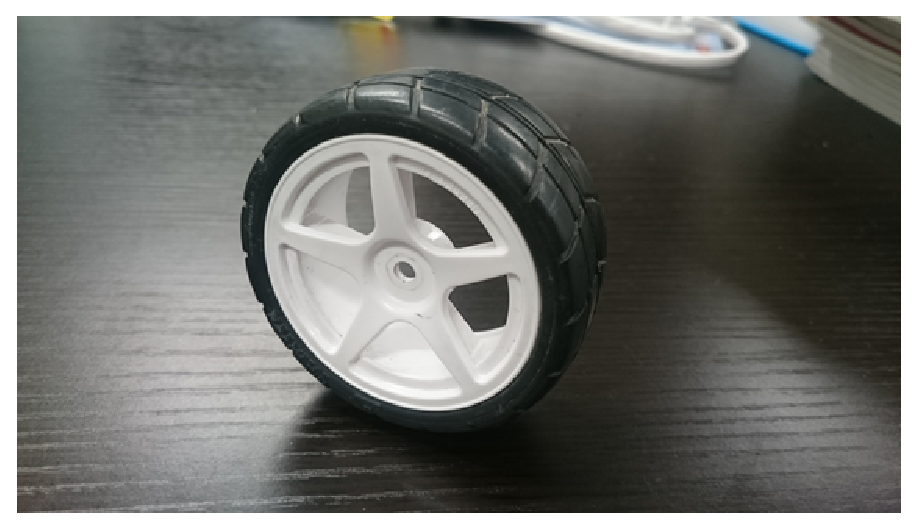
\includegraphics[width=1.0\hsize]{picture/kuwano5.eps}
    \caption{一号機のタイヤ}
    \label{kuwano5}
  \end{center}
\end{figure}

\begin{figure}[t]
  \begin{center}
    \includegraphics[width=1.0\hsize]{picture/kuwano6.eps}
    \caption{二号機のナロータイヤ}
    \label{kuwano6}
  \end{center}
\end{figure}

\end{document}